\chapter{Appendix}

\section{PCB layout}
\begin{figure}[htb]
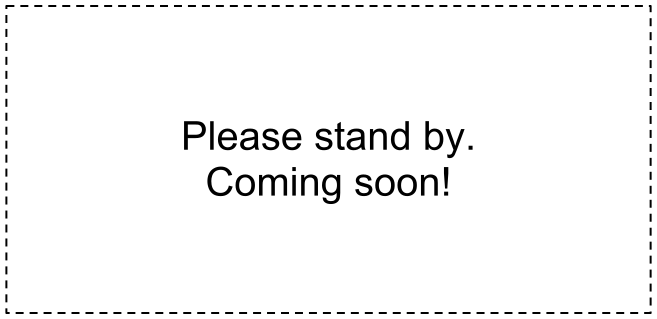
\includegraphics[width=\columnwidth]{Images/dummy}
%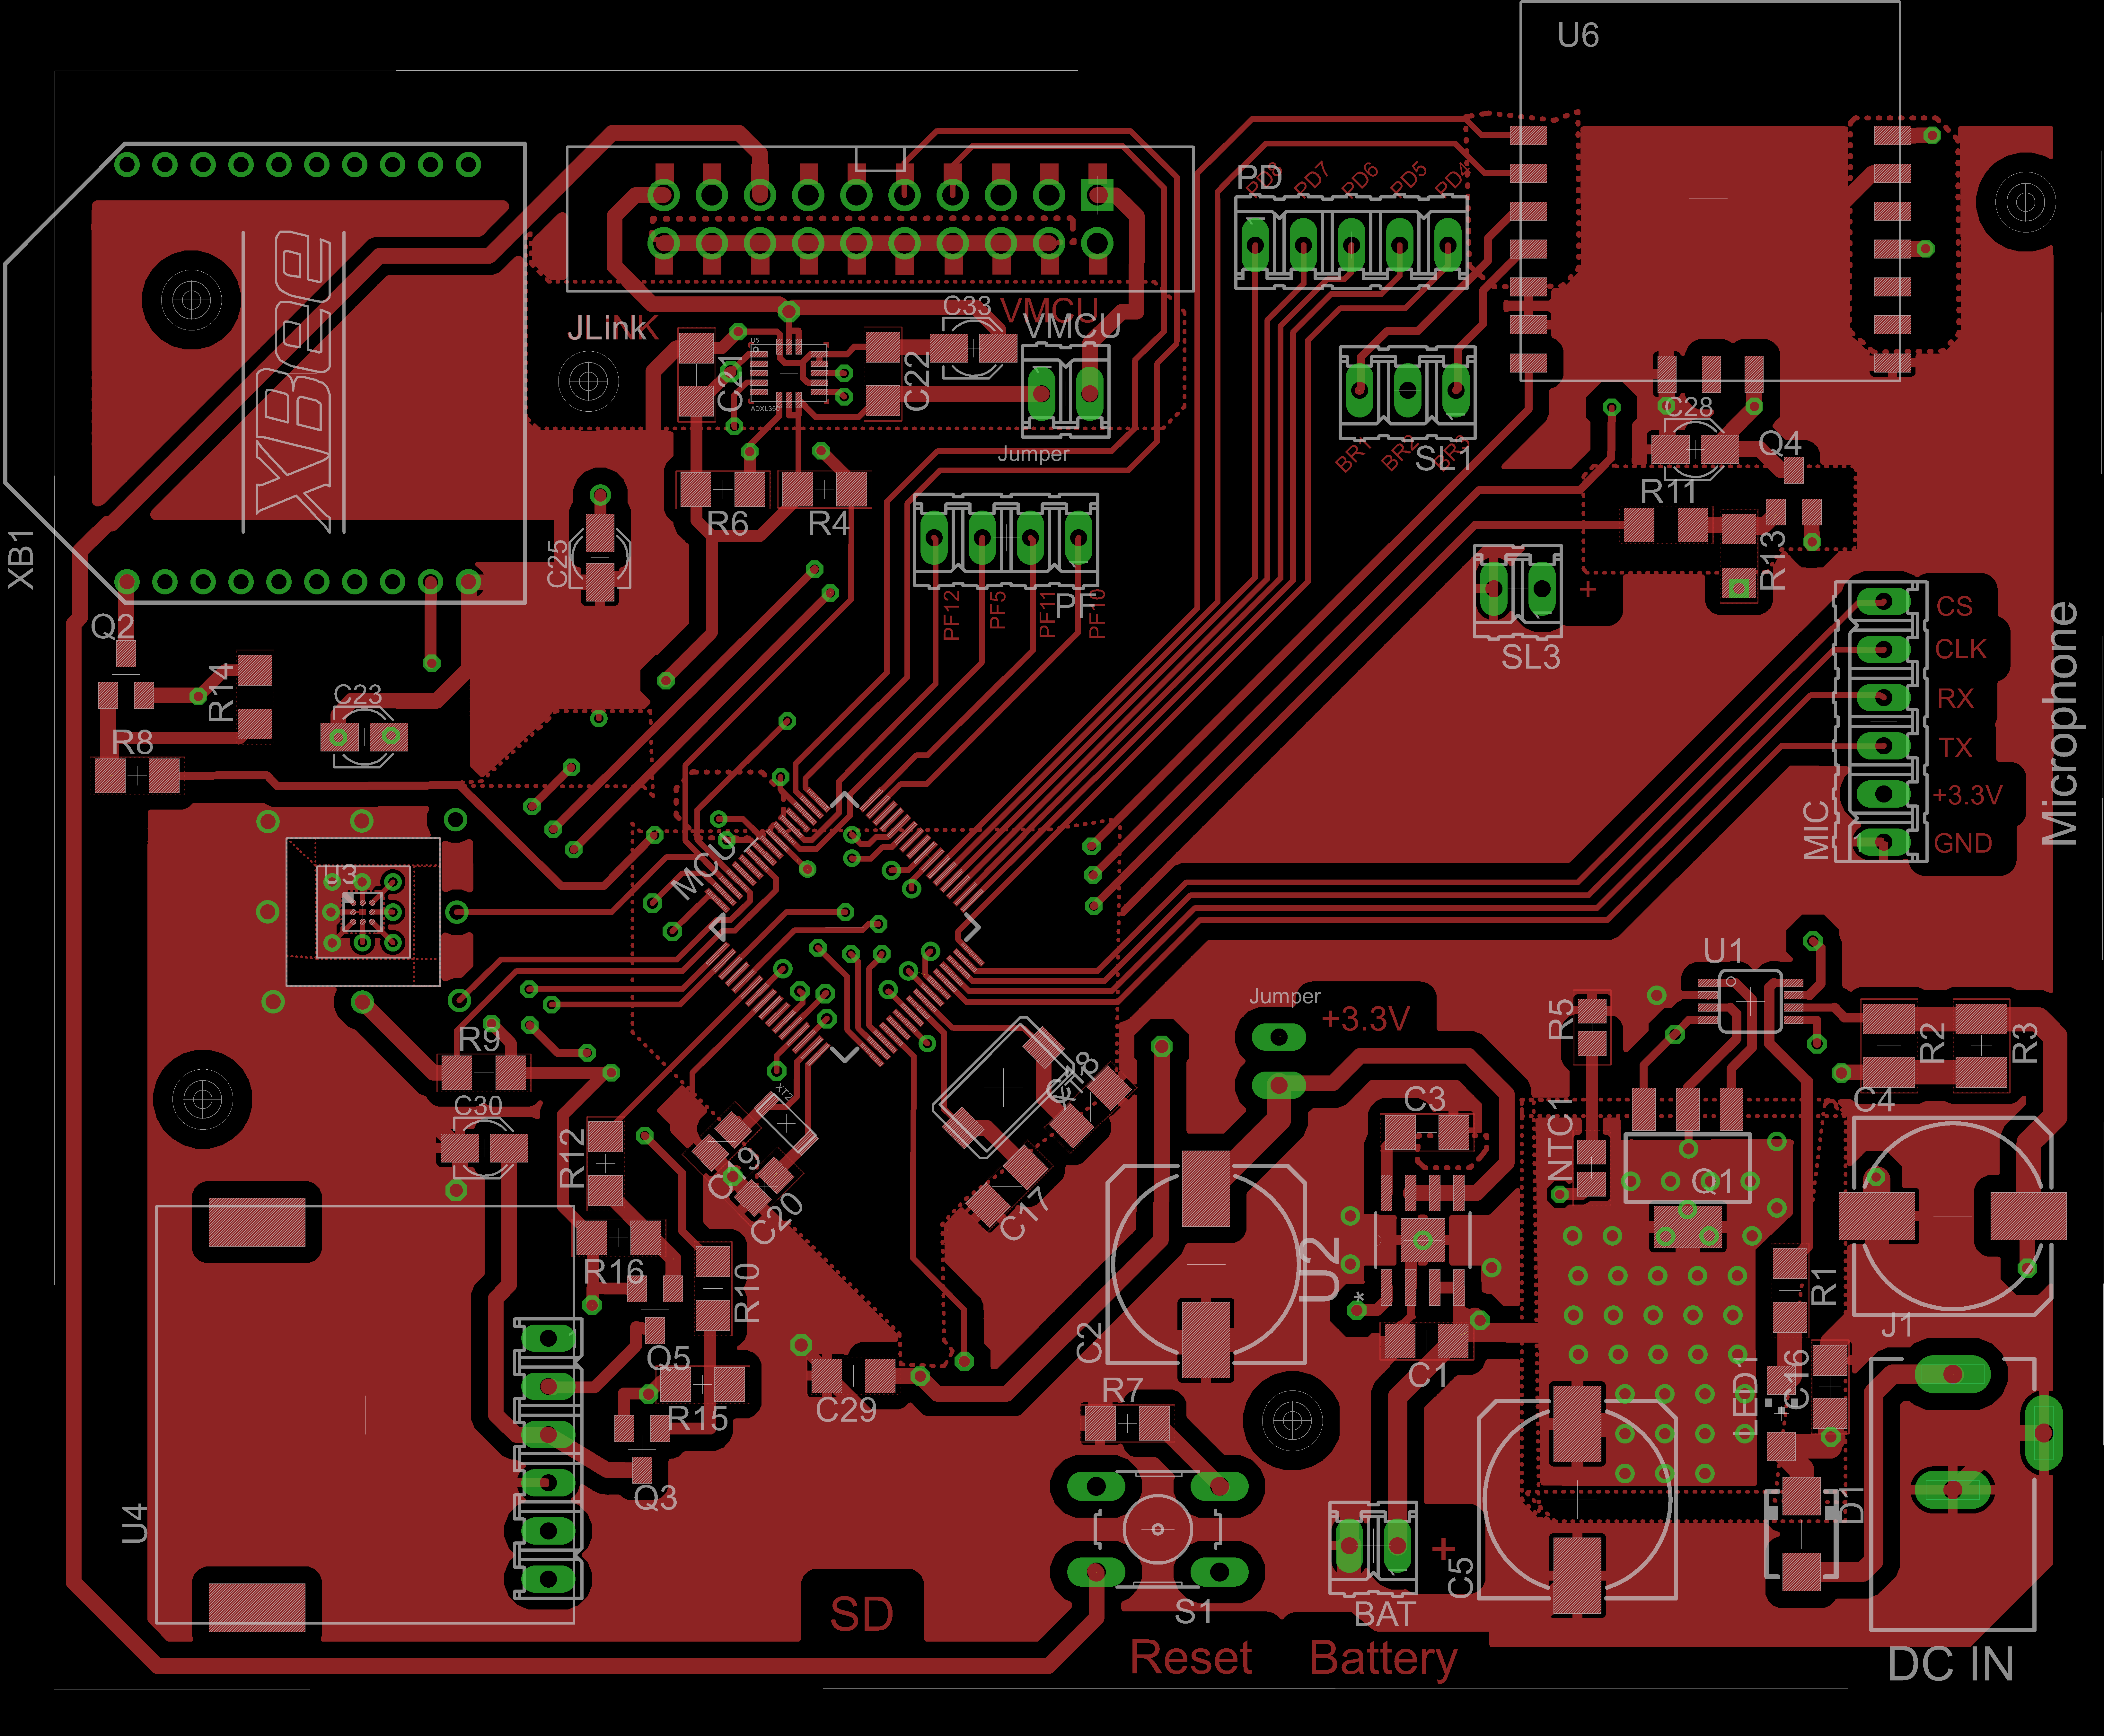
\includegraphics[width=\columnwidth]{Images/pcb_layout_top}
\caption{PCB layout top}
\label{fig:pcb_layout_top}
\end{figure}

\begin{figure}[htb]
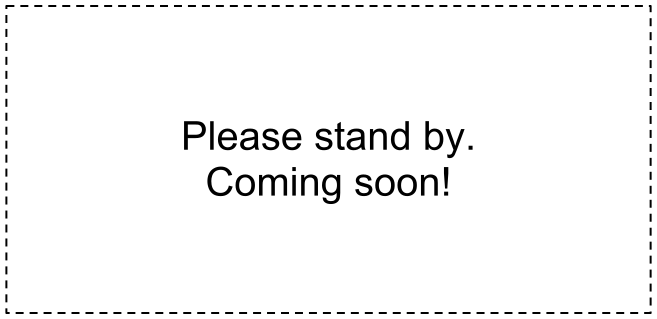
\includegraphics[width=\columnwidth]{Images/dummy}
%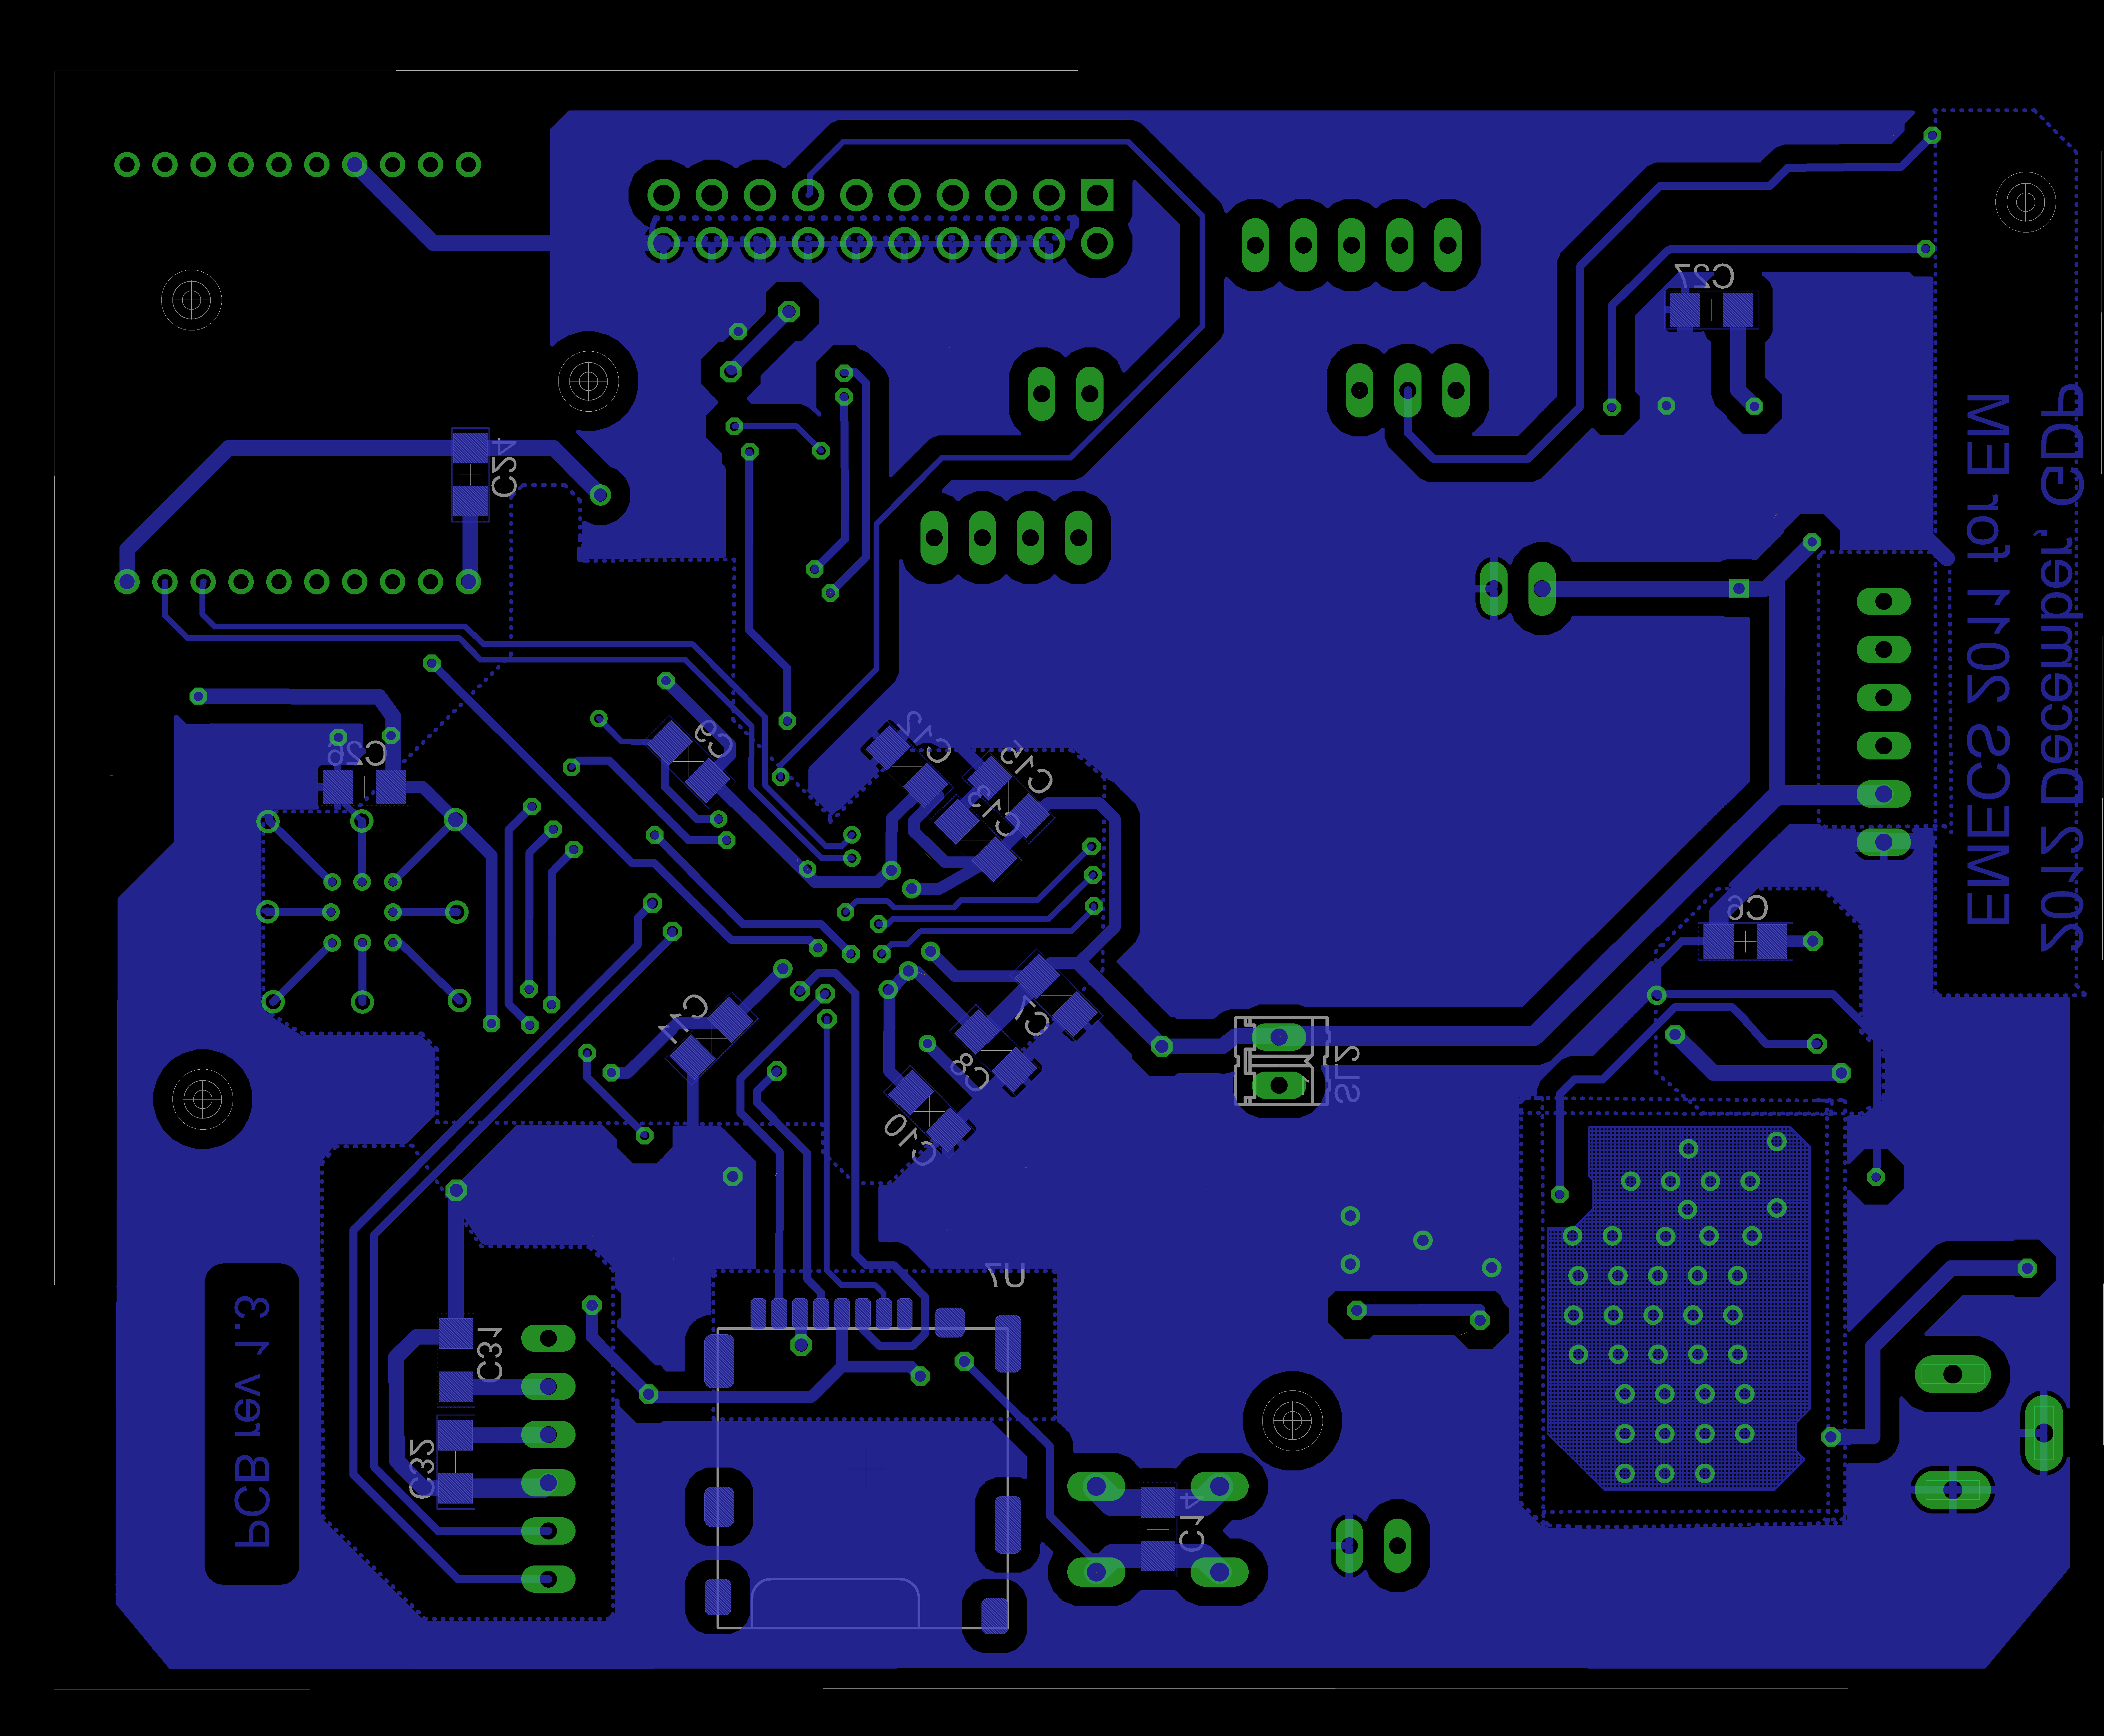
\includegraphics[width=\columnwidth]{Images/pcb_layout_bottom}
\caption{PCB layout bottom}
\label{fig:pcb_layout_bottom}
\end{figure}

\begin{figure}[htb]
\centering
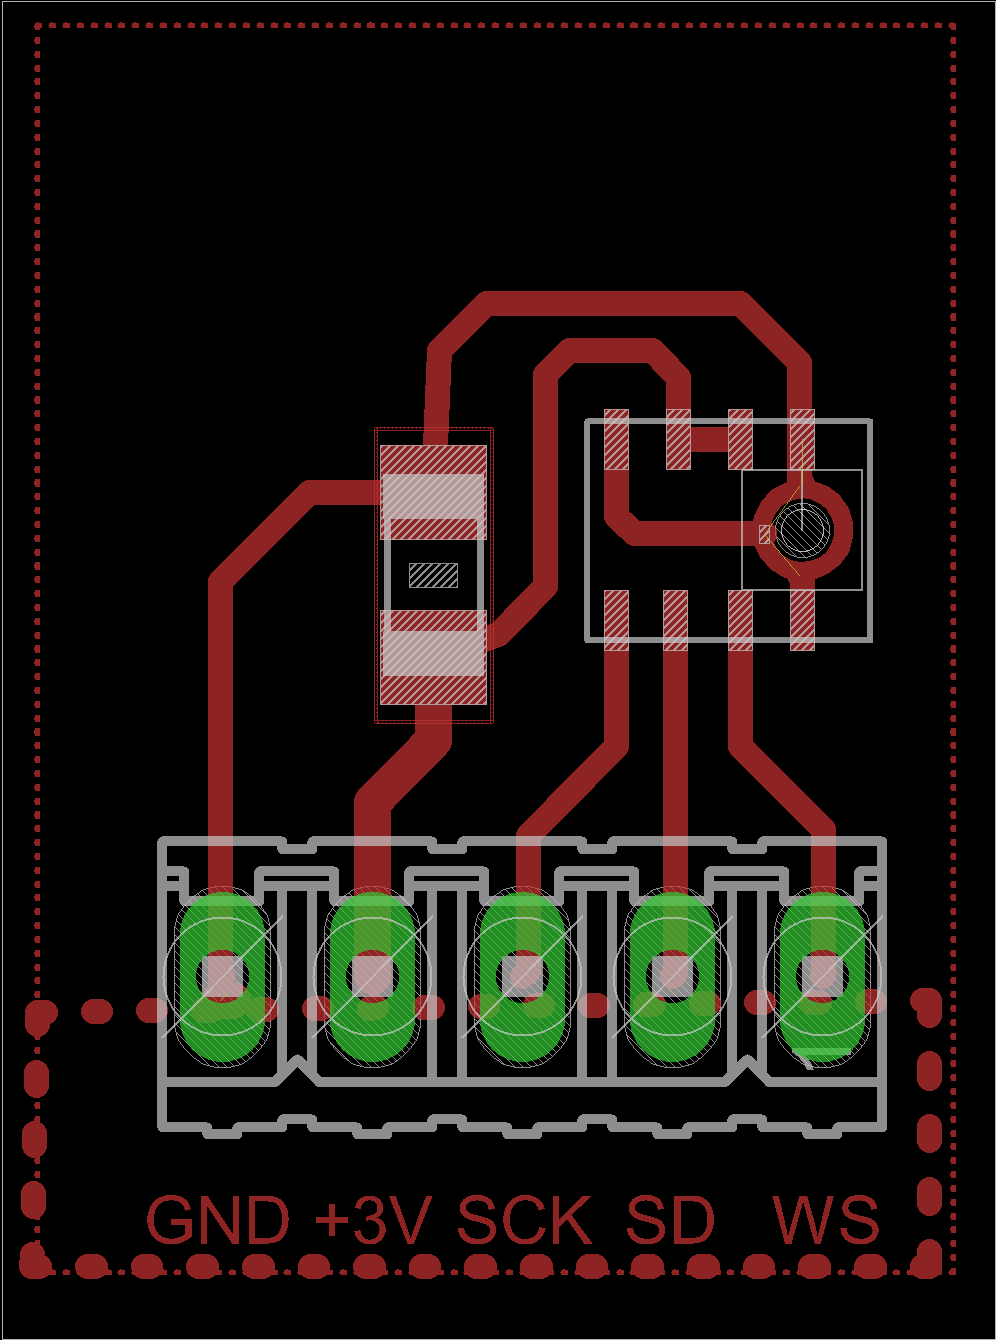
\includegraphics[width=0.4\columnwidth]{Images/pcb_layout_mic}
\caption{PCB layout microphone}
\label{fig:pcb_layout_mic}
\end{figure}

\clearpage

\section{PCB schematics}
\label{sec:pcb_schematics}
\begin{itemize}
\item PCB schematics: Power and LDO \ref{fig:pcb_schematics_6}
\item PCB schematics: MCU, decoupling, oscillators and reset \ref{fig:pcb_schematics_4}
\item PCB Schematics: ANT, XBee and SD \ref{fig:pcb_schematics_1}
\item PCB Schematics: I2C and GPS \ref{fig:pcb_schematics_3}
\item PCB Schematics: Debug headers and microphone \ref{fig:pcb_schematics_2}
\item PCB schematics: Microphone \ref{fig:pcb_schematics_5}
\end{itemize}


\begin{figure}[htb]
\centering
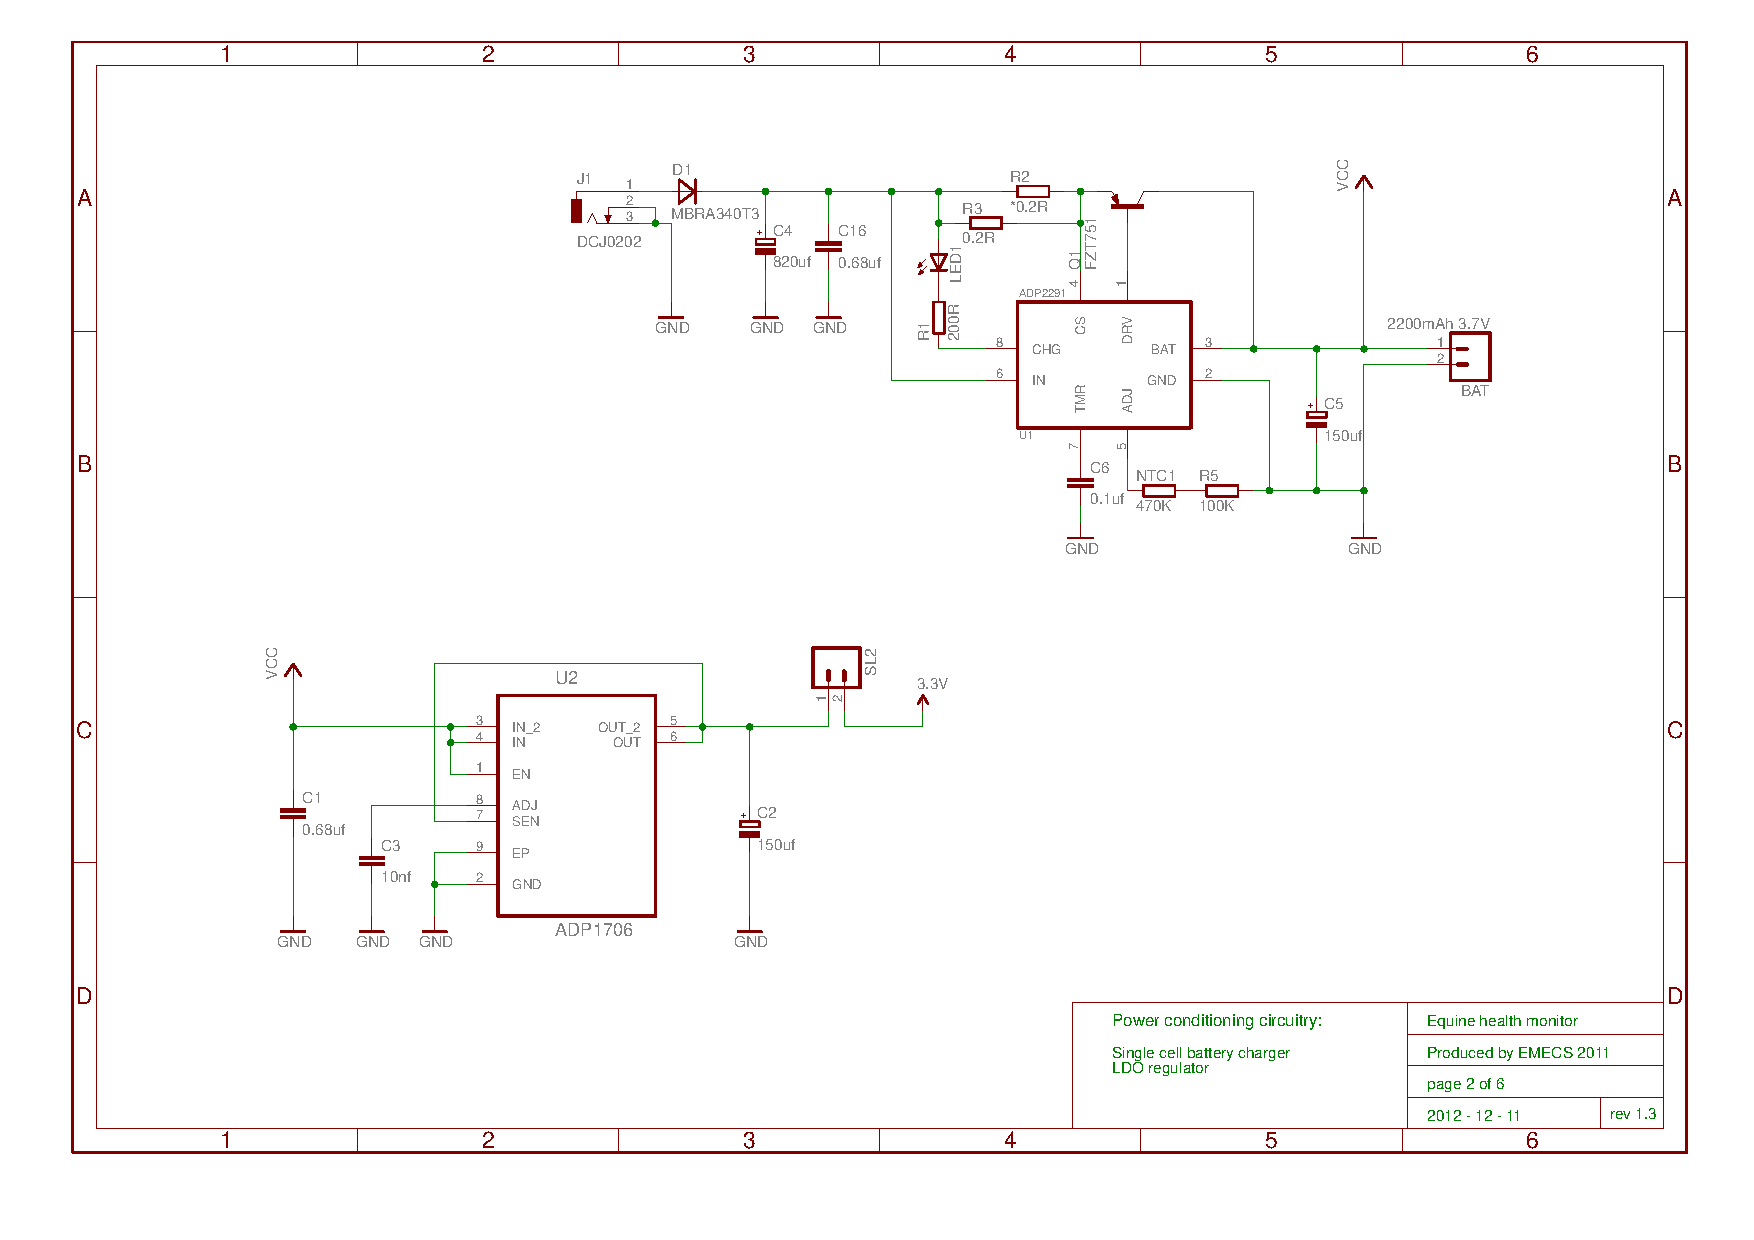
\includegraphics[width=\columnwidth]{Images/pcb_power_ldo}
\caption{PCB schematics: Power and LDO}
\label{fig:pcb_schematics_6}
\end{figure}

\begin{figure}[htb]
\centering
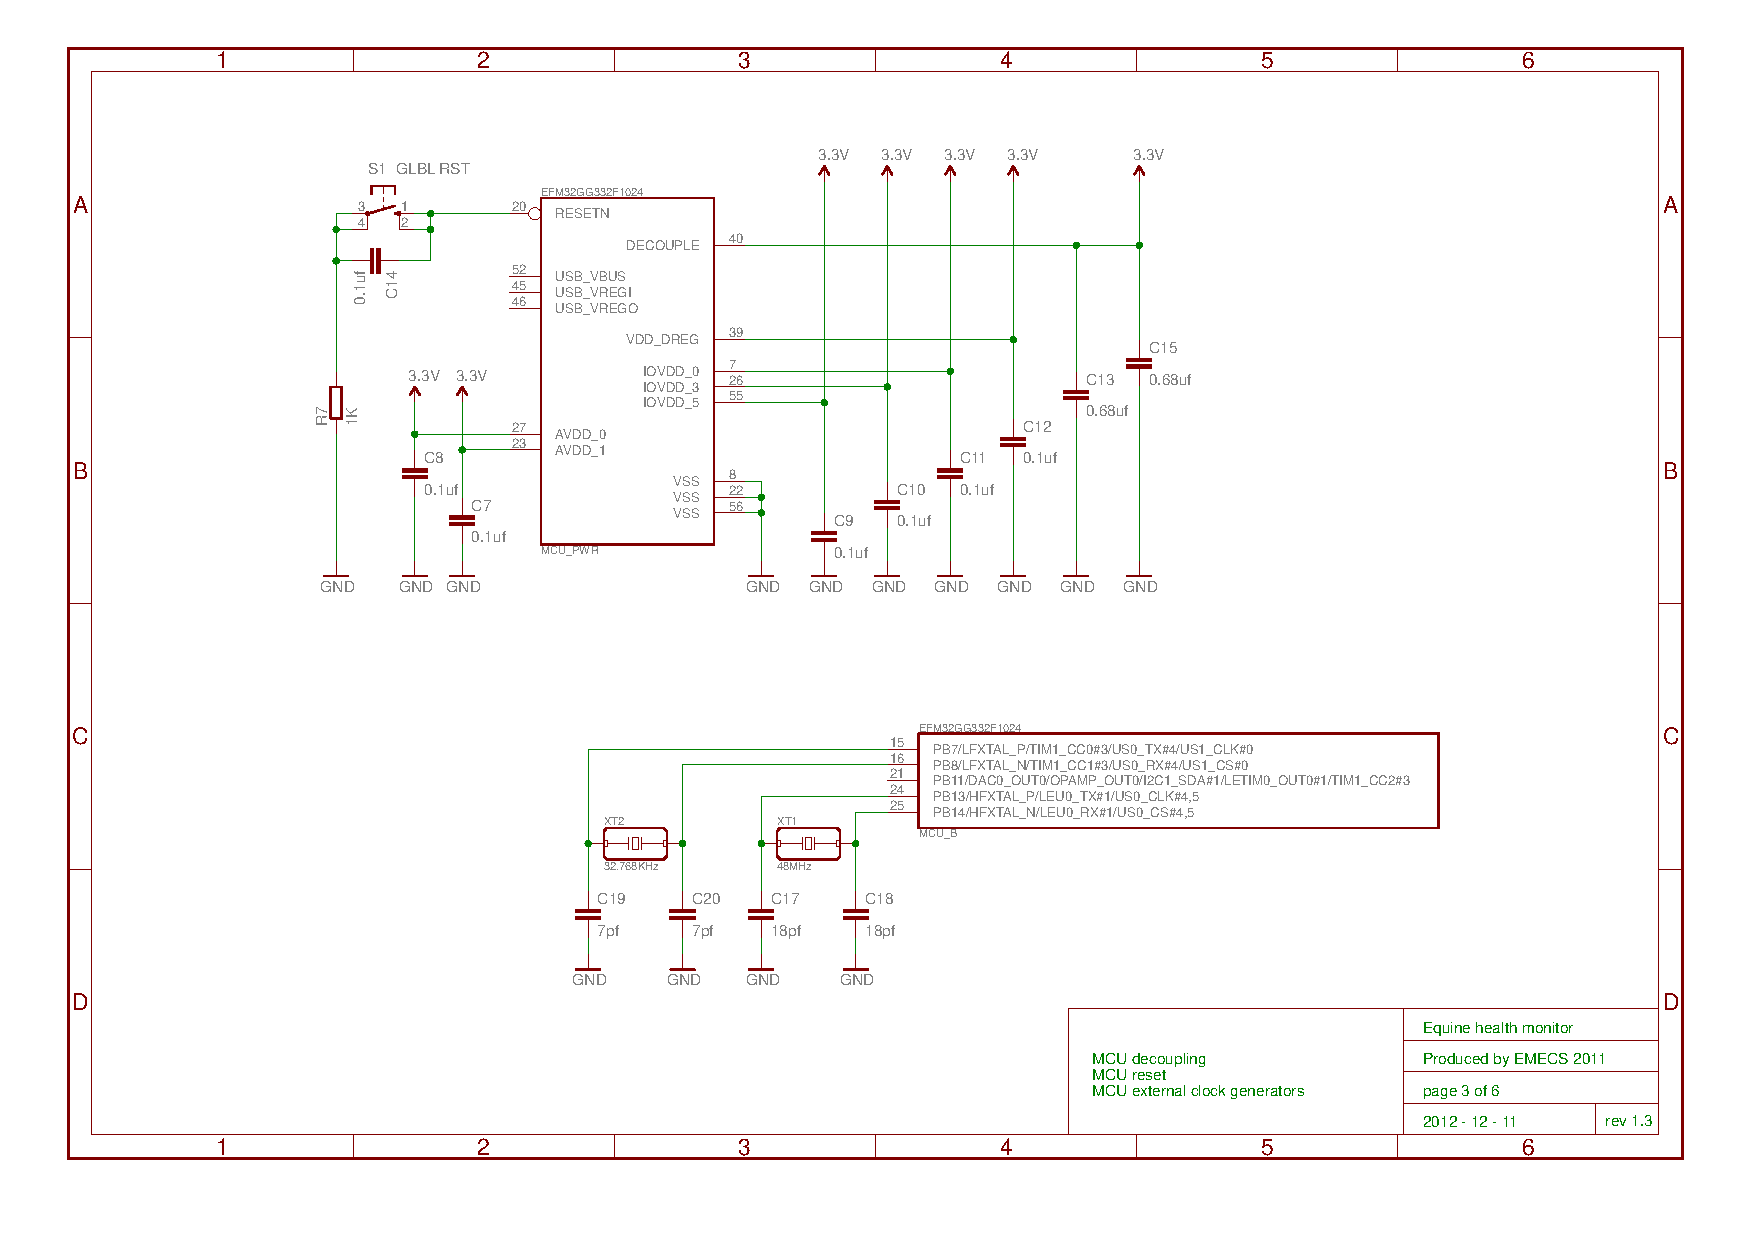
\includegraphics[width=\columnwidth]{Images/pcb_mcu_osc_reset}
\caption{PCB schematics: MCU, decoupling, oscillators and reset}
\label{fig:pcb_schematics_4}
\end{figure}

\begin{figure}[htb]
\centering
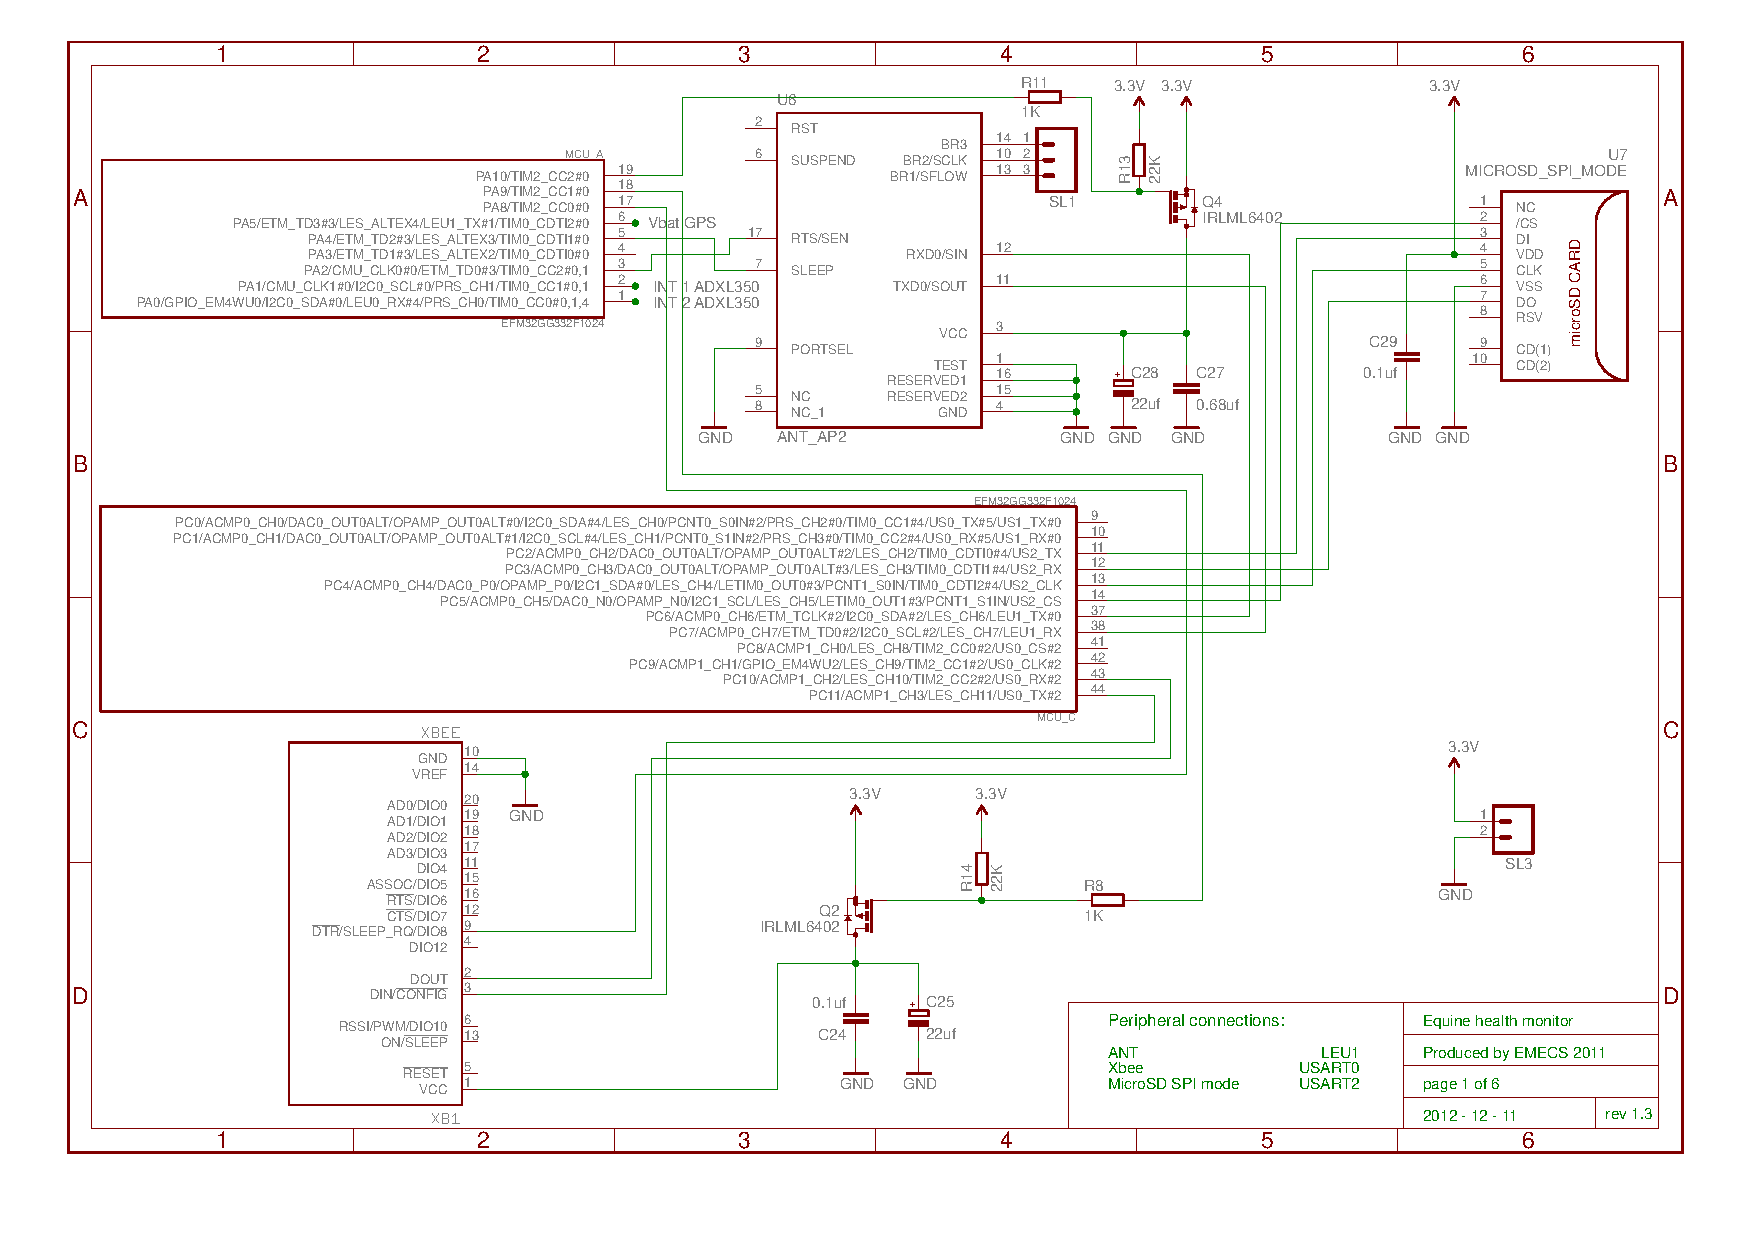
\includegraphics[width=\columnwidth]{Images/pcb_ant}
\caption{PCB schematics: ANT, XBee and SD}
\label{fig:pcb_schematics_1}
\end{figure}

\begin{figure}[htb]
\centering
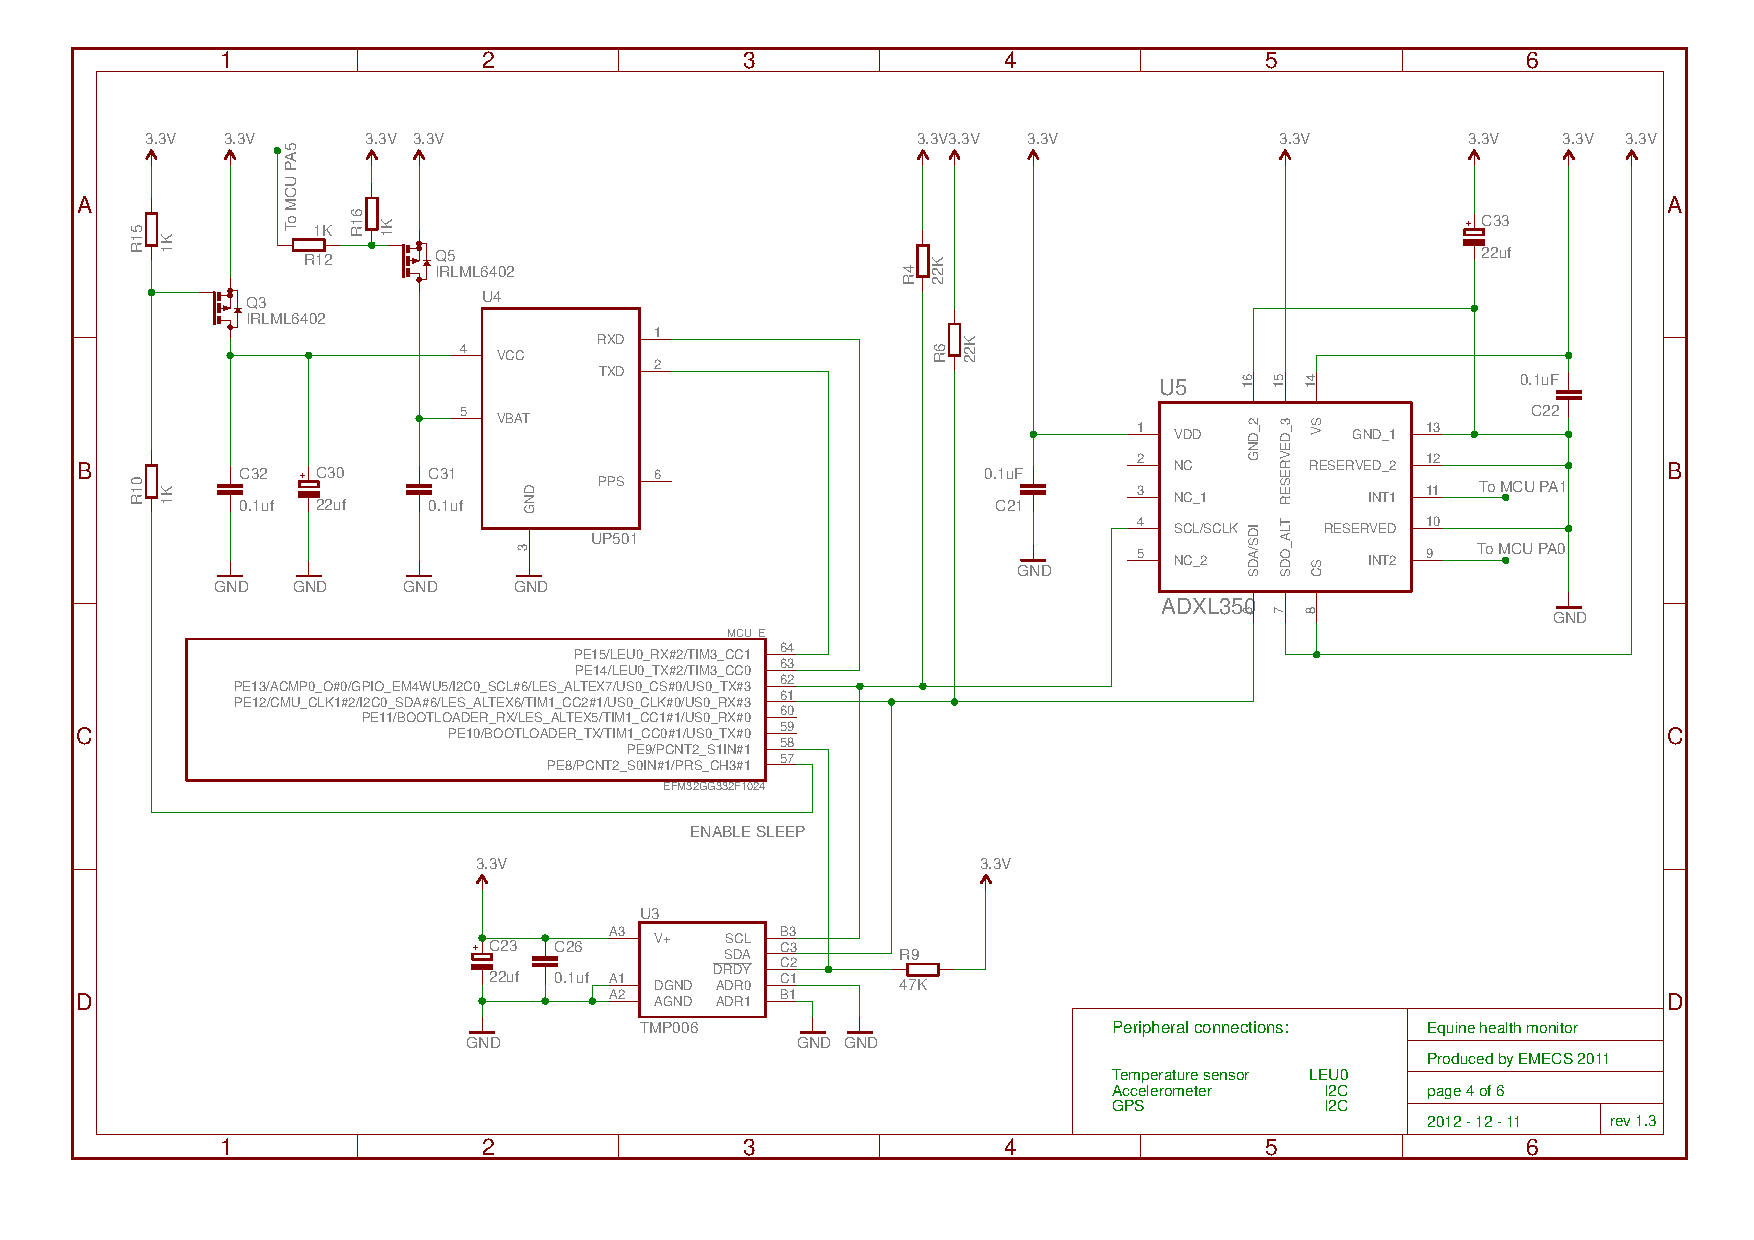
\includegraphics[width=\columnwidth]{Images/pcb_i2c_gps}
\caption{PCB schematics: I2C and GPS}
\label{fig:pcb_schematics_3}
\end{figure}

\begin{figure}[htb]
\centering
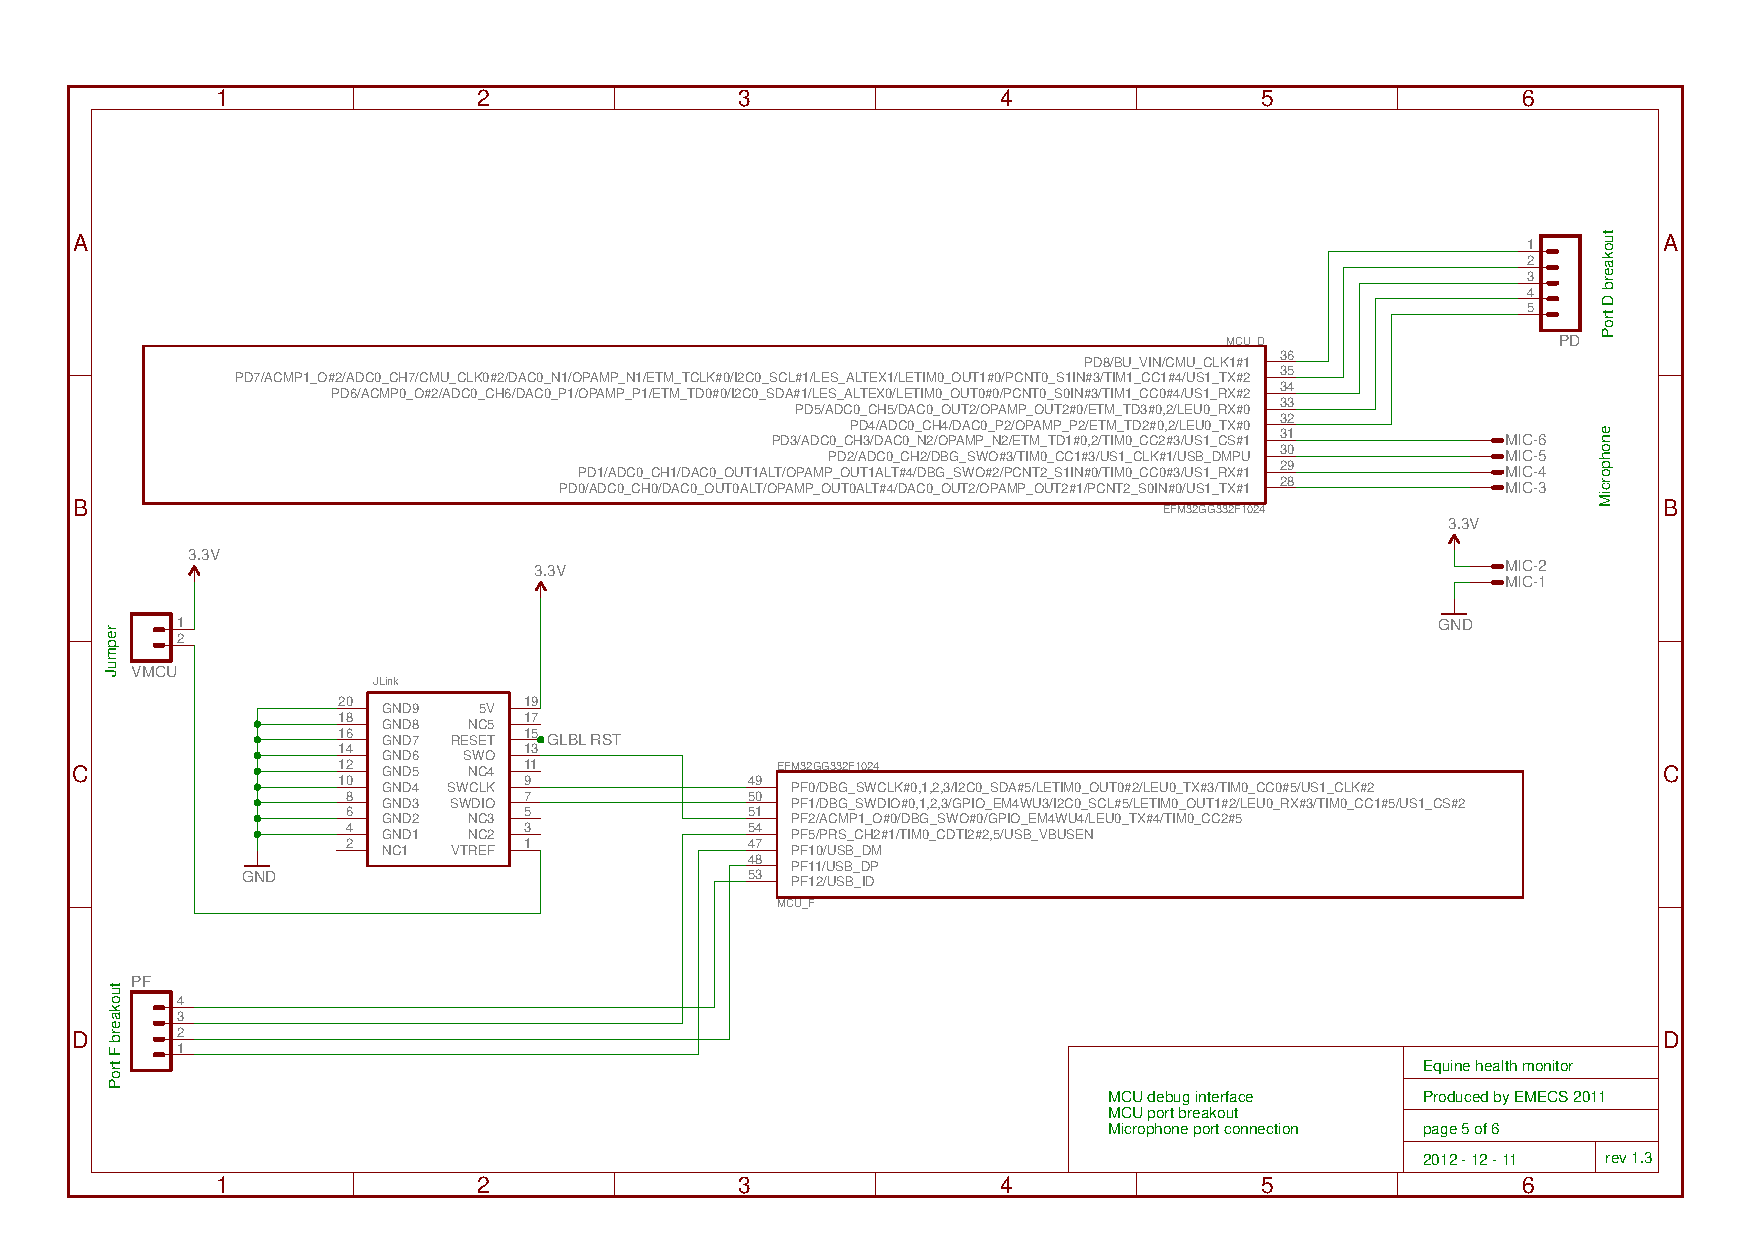
\includegraphics[width=\columnwidth]{Images/pcb_debug_mic}
\caption{PCB schematics: Debug headers and microphone}
\label{fig:pcb_schematics_2}
\end{figure}




\begin{figure}[htb]
\centering
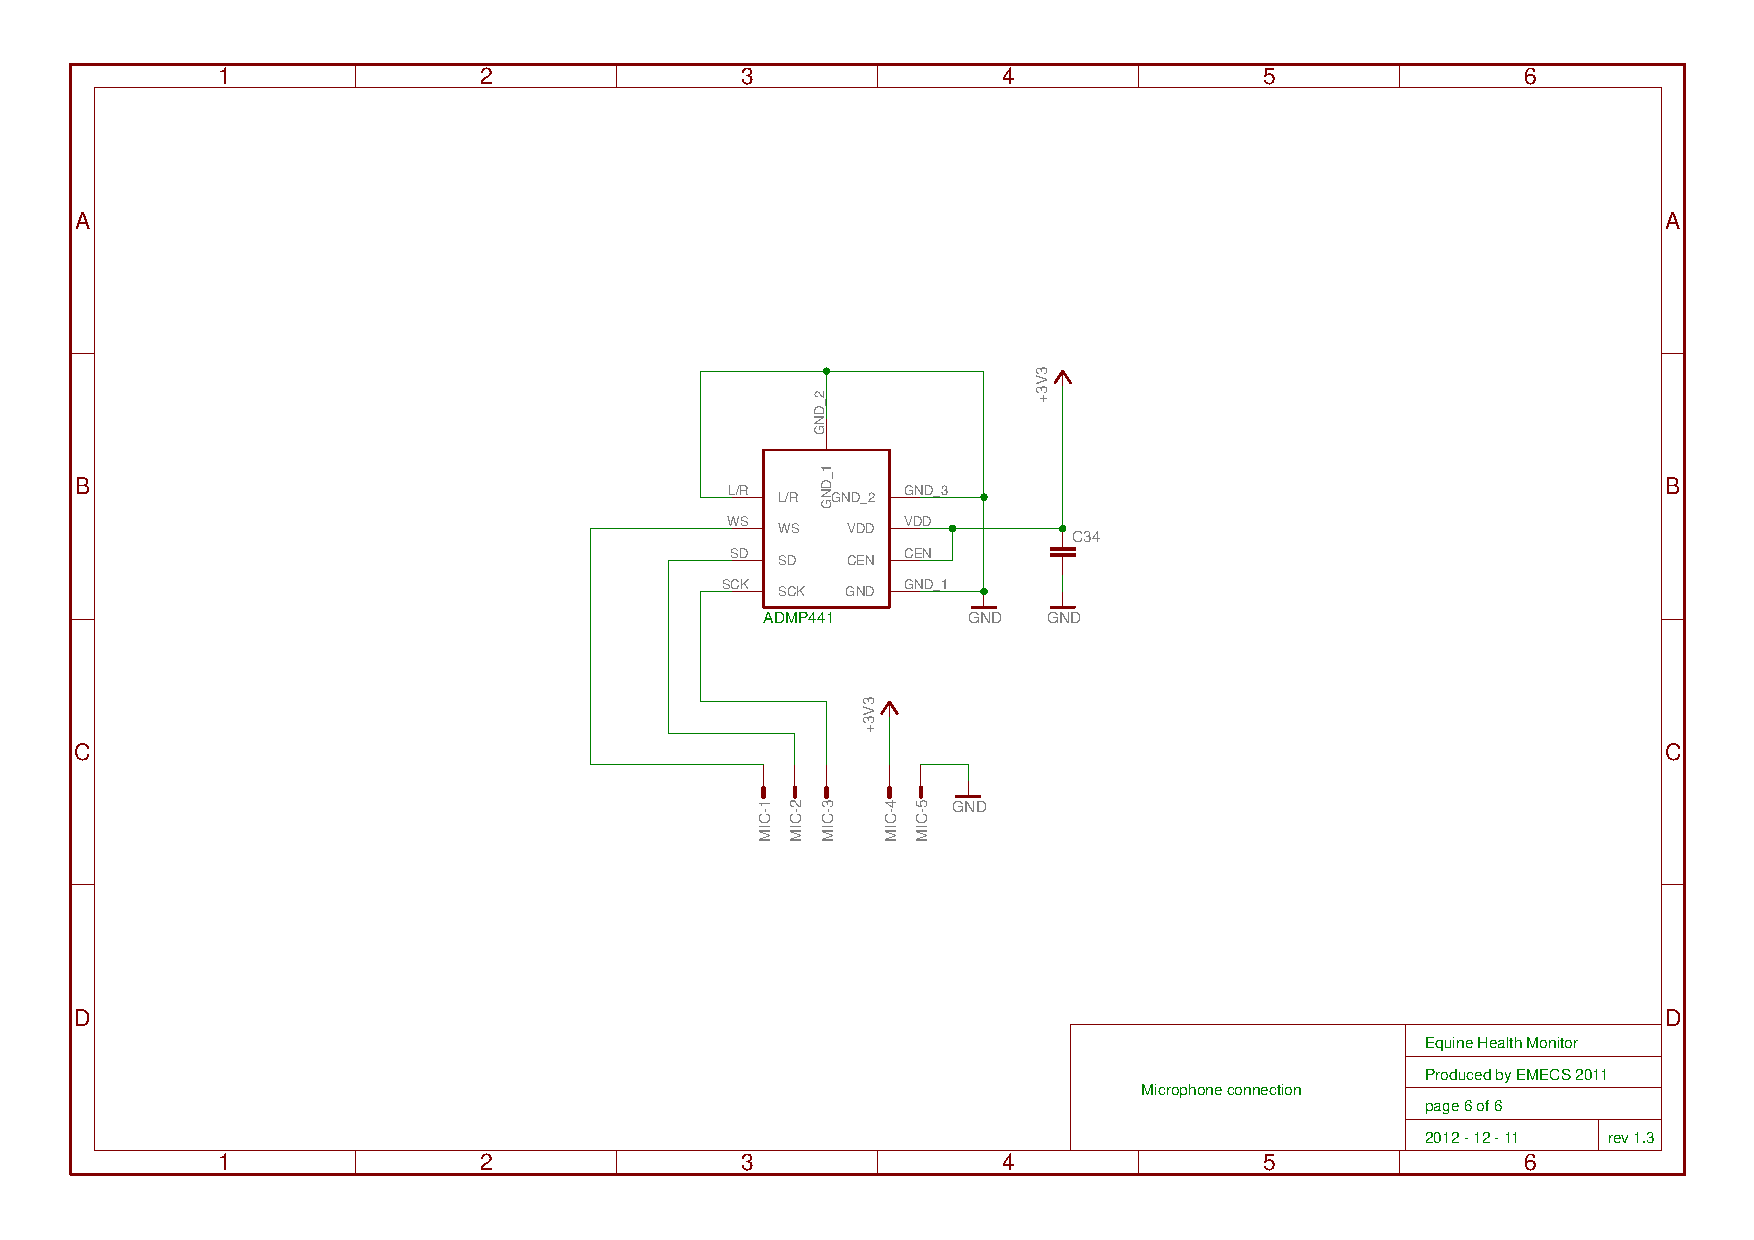
\includegraphics[width=\columnwidth]{Images/pcb_mic}
\caption{PCB schematics: Microphone}
\label{fig:pcb_schematics_5}
\end{figure}






\clearpage
\section{Gantt Chart}
\label{sec:gantt_chart}
\begin{figure}[htb]
\centering
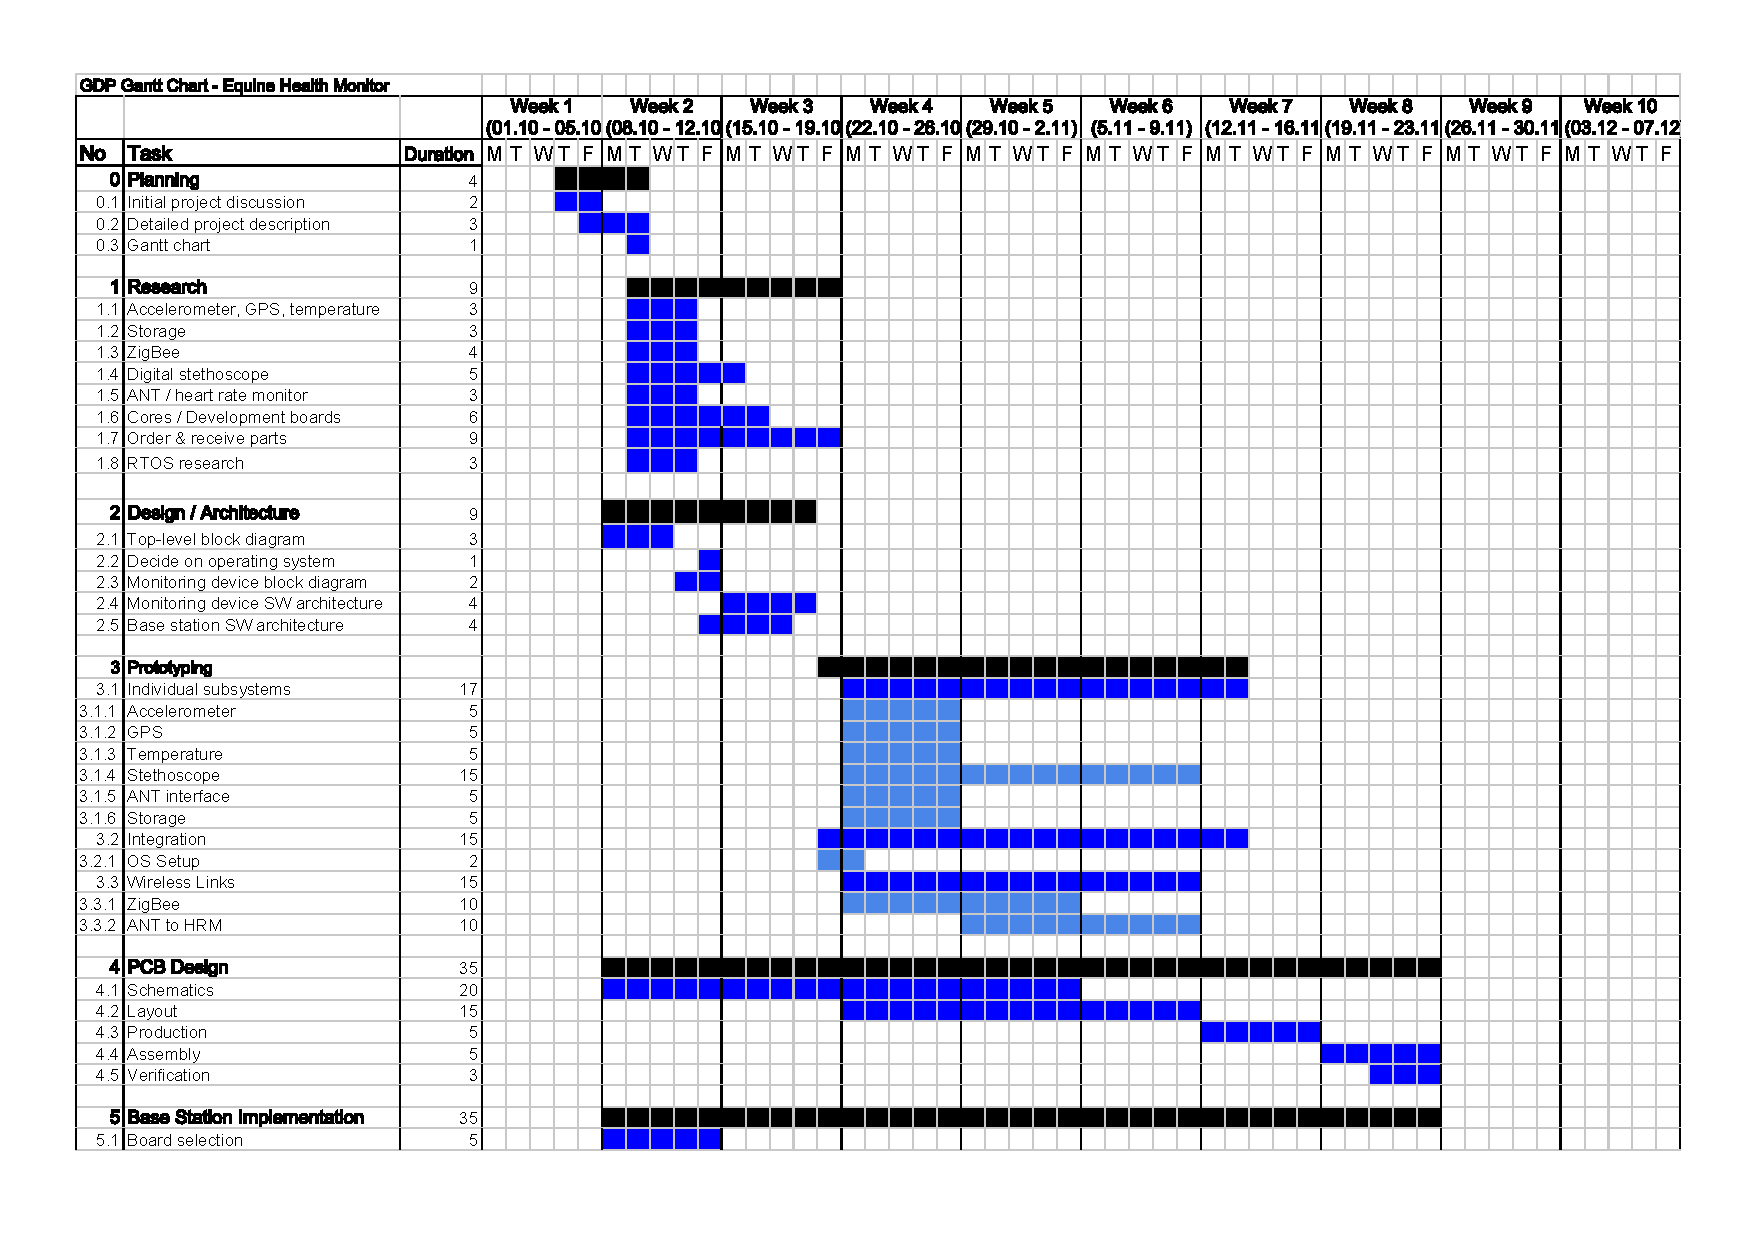
\includegraphics[angle=90, width=0.9\columnwidth]{Data/gantt_chart}
\caption{Gantt Chart}
\label{fig:gantt_chart}
\end{figure}

\clearpage

\section{Task distribution}
\label{sec:task_distribution}
\TODO{}


\section{Task break-down}
\label{sec:task_breakdown}
\TODO{}


\section{Price List}
\label{sec:price_list}
Please refer to table \ref{tab:pricelist}.
\begin{table}[hb]
\centering
\begin{tabular}{|l|l|l|}\hline%
\bfseries Component & \bfseries Price (GBP) & \bfseries Retail Price (GBP)\\\hline
\csvreader[ %
	head to column names,
	late after line=\\
]{Data/price_list.csv}{}%
{\Component & \Price & \Retail}%
\hline
\end{tabular}
\caption{Component Price List}
\label{tab:pricelist}
\end{table}
\clearpage

\section{Part List}
\label{sec:part_list}
Please refer to table \ref{tab:part_list_1} and \ref{tab:part_list_2} for the part list. 

\begin{sidewaystable}
\scriptsize
\begin{tabular}{|l|l|l|m{2.3cm}|l|l|l|}\hline%
\bfseries Part & \bfseries Value & \bfseries Device & \bfseries Description & \bfseries Package & \bfseries Manufacturer & \bfseries Man. part nr. \\\hline
\csvreader[ %
	head to column names,
	late after line=\\
]{Data/partlist_part1.csv}{}%
{\Part & \Value & \Device & \Description & \Package & \Manufacturer & \PartNr}%
\hline
\end{tabular}
\caption{Part list part 1}
\label{tab:part_list_1}
\end{sidewaystable}

\begin{sidewaystable}
\scriptsize
\begin{tabular}{|l|l|l|m{2.3cm}|l|l|l|}\hline%
\bfseries Part & \bfseries Value & \bfseries Device & \bfseries Description & \bfseries Package & \bfseries Manufacturer & \bfseries Man. part Nr. \\\hline
\csvreader[head to column names,
late after line=\\
]{Data/partlist_part2.csv}{}%
{\Part & \Value & \Device & \Description & \Package & \Manufacturer & \PartNr}%
\hline
\end{tabular}
\caption{Part list part 2}
\label{tab:part_list_2}
\end{sidewaystable}
\clearpage

\section{Fieldtrip}
\subsection{Gut Sound Recordings}
\label{sec:gut_sound_recordings}
Please refer to table \ref{tab:gut_sound_recordings}
\begin{table}
\centering
\small
\begin{tabular}{|c|l|p{2cm}|l|}\hline%
\bfseries \# & \bfseries Description & \bfseries Part of the abdomen & \bfseries Link \\\hline
\csvreader[head to column names,
late after line=\\
]{Data/gut_sound_recordings.csv}{}%
{\Horse & \Type & \Part & \Link}%
\hline
\end{tabular}
\caption{Gut sound recordings}
\label{tab:gut_sound_recordings}
\end{table}


\subsection{Pictures}
Please refer to figure \ref{fig:field_trip_a} and \ref{fig:field_trip_b}.
\begin{figure}[htb]
\centering
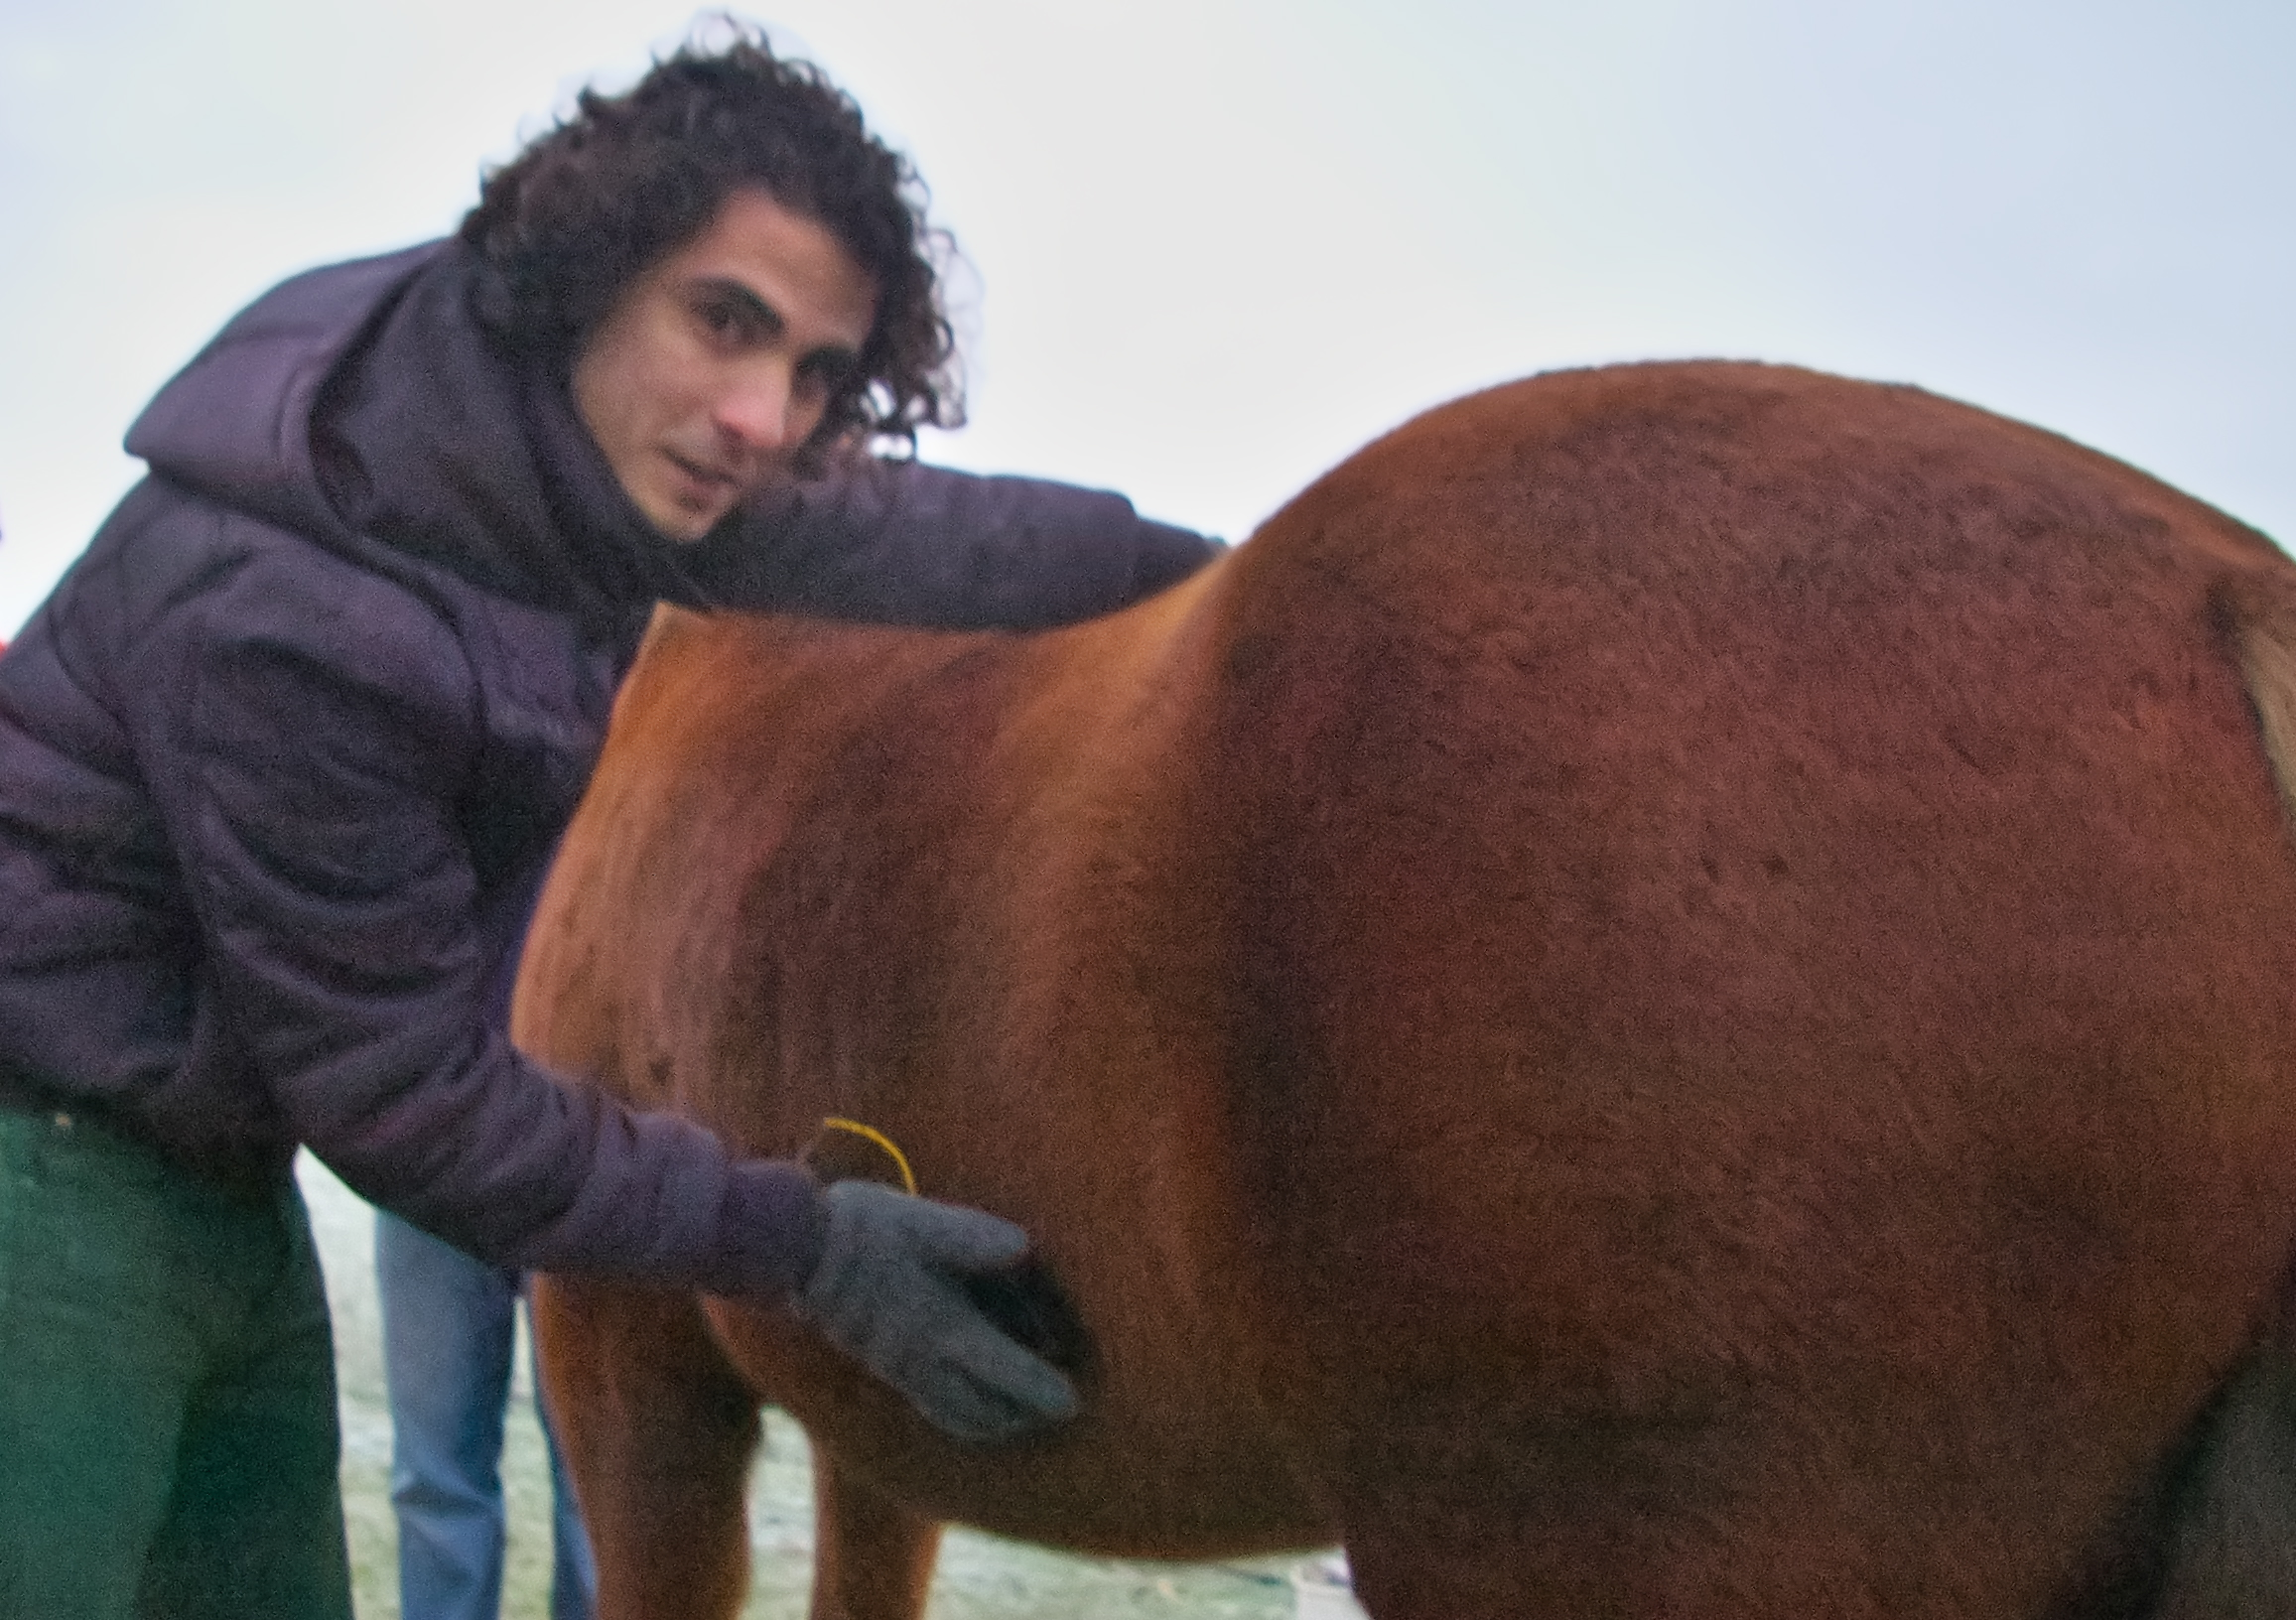
\includegraphics[width=0.7\columnwidth]{Images/field_trip_a.jpg}
\caption{Photo: Field trip (a)}
\label{fig:field_trip_a}
\end{figure}
\begin{figure}[htb]
\centering
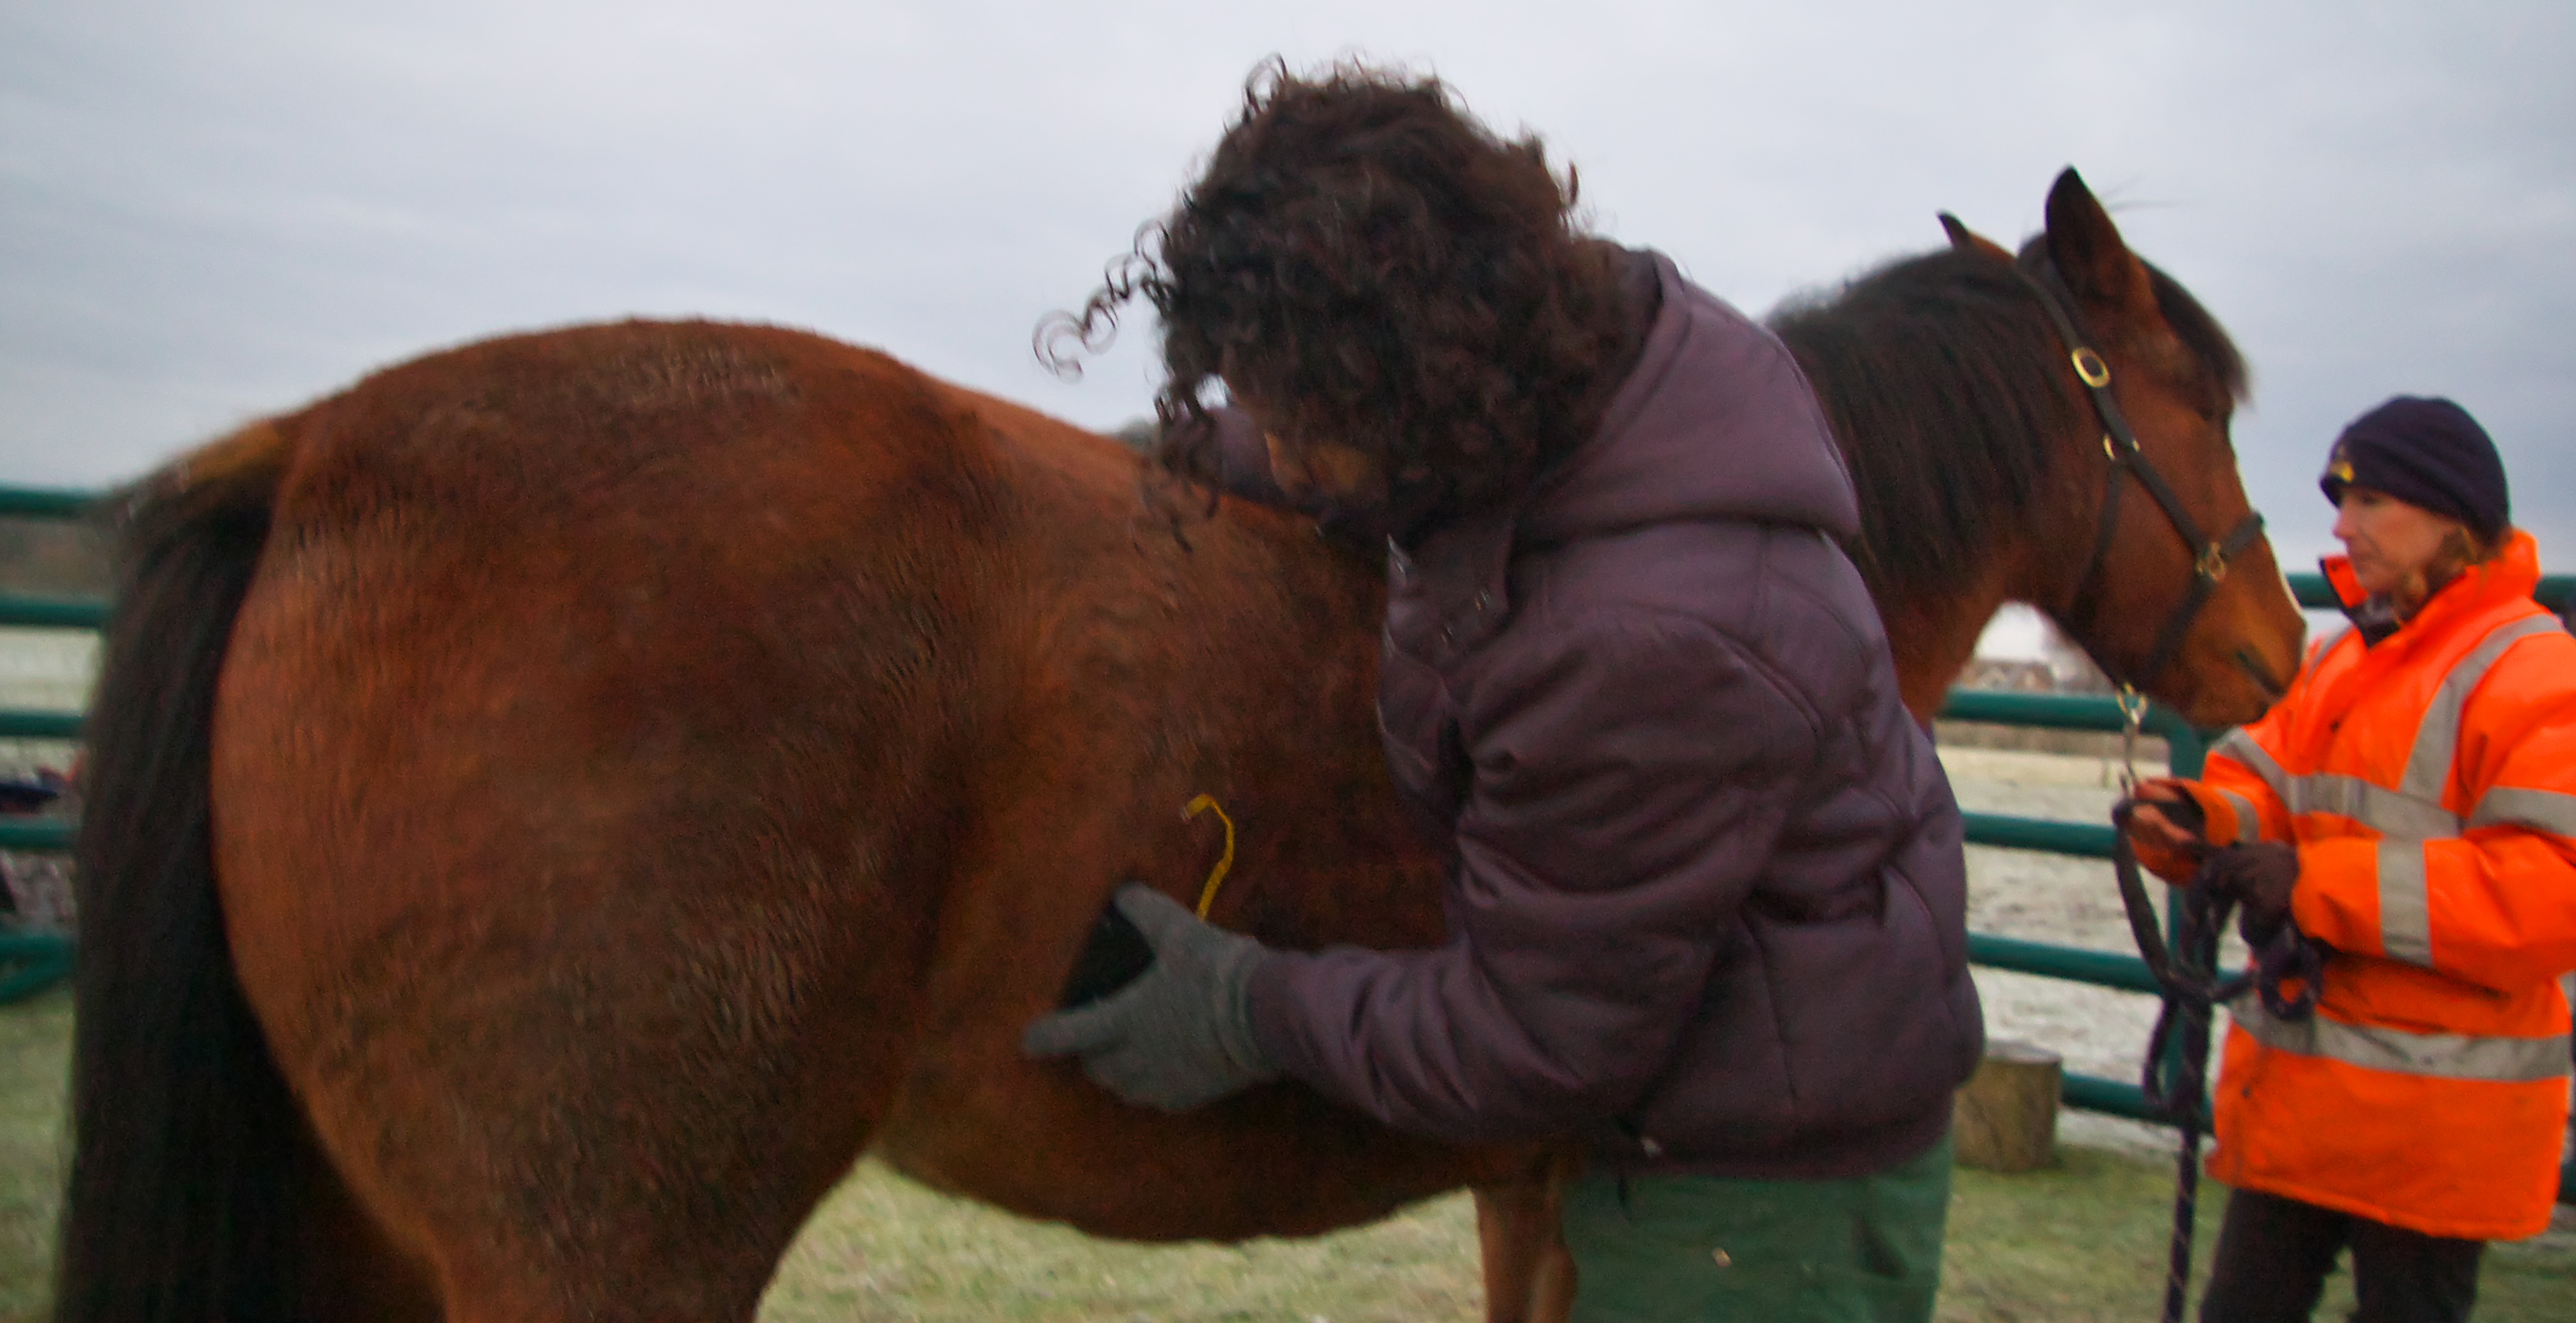
\includegraphics[width=0.7\columnwidth]{Images/field_trip_b.jpg}
\caption{Photo: Field trip (b)}
\label{fig:field_trip_b}
\end{figure}

